\chapter*{Introduction}
\addcontentsline{toc}{chapter}{Introduction}

These notes, that I won't consider a book because of its informality, were born as an idea after ending the course, Álgebra IV in ESFM IPN, unsatisfied. That isn't saying that I hated Dr. Hugo's classes. I love him. But the contents were not the best for my idea of an algebra IV course focused on set theory.

These notes are meant to help understand and clarify a lot of things not included in the course I took. Is not some kind of tortuous book that some gifted individuals can read, I'm not that good. It is written in a way that makes the part of the course almost completely independent of the first chapter. However, for a better understanding on what set theory is constructed over, it should be read at least once or twice because my writing, as a lot of people can confirm, is not the best.

The plan is, to clarify things about logic, especially for first order logic that is what set theory is usually developed over. But also, it works as prerequisites for further topics on set theory and what interests me most, foundations of mathematics.
Next chapter deals with the usual course on set theory, giving axioms and its interpretations, proving statements about relations, functions, equivalence, unicity, existence, etc. The final stop for this chapter are the real numbers and its properties constructed via sets.
A further study on set theory, topics like cardinality, axiomatical systems and combinatorics are, aside from interesting, sometimes very necessary for further topics on algebra, analysis, etc. Not indispensable, yes, but really good to know for them.
A chapter about structures is then introduced, trying to get to universal algebra and an introduction to category theory via set theory.
And finally, a chapter on the foundations for the curious mind that wants to waste some time on interesting things like foundational category theory, drug addict thinking in metamathematics and a formalization of logic via mathematics, a seemingly circular foundation. Also, with sections that are of my interest, like type theory and philosophy of mathematics.

All of this, in my opinion, conforms an overloaded course on set theory, and should be taken very selectively and with a grain of salt. I'm just a but a dumb student right now.

\begin{figure}[h]
	\centering
	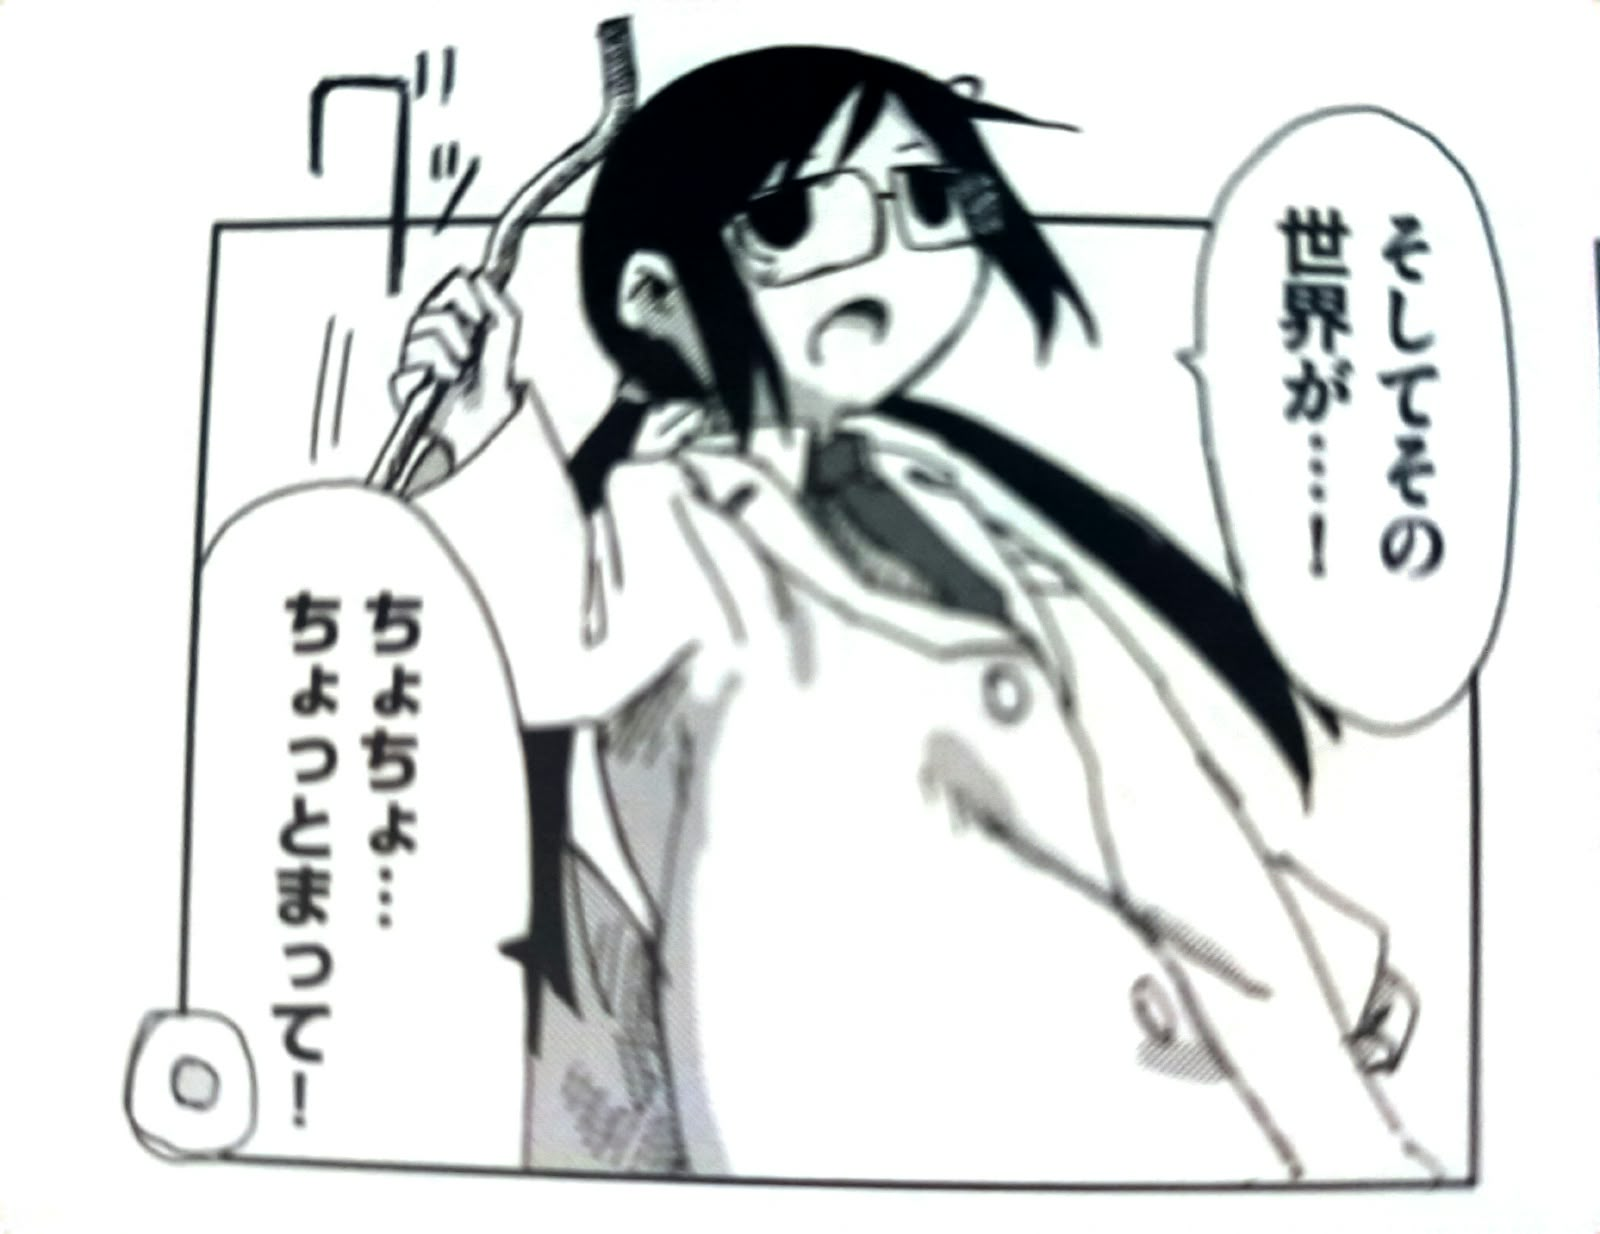
\includegraphics[width=10cm, height=8cm]{img/soshite.jpeg}
\end{figure}
